\documentclass[11pt]{article}
\usepackage[utf8]{inputenc}
\usepackage{graphicx}
\usepackage{subcaption}
\usepackage{amsmath}
\usepackage{geometry}
\usepackage{caption}
\usepackage{hyperref}
\usepackage{float}
\usepackage{placeins}

\geometry{a4paper, margin=1in}
\title{trajectories Evaluation Using Evo}
\author{}
\date{}

\begin{document}

\maketitle

\section{Introduction}

This document presents the evaluation results, which was estimated using odometry and compared against a ground truth trajectories (\texttt{motive\_tracking\_pose}) obtained from a motion capture system. The analysis was performed using the \texttt{evo} toolkit, a popular library for evaluating SLAM and odometry results.

\section{trajectories Comparison}

\begin{figure}[H]
    \centering
    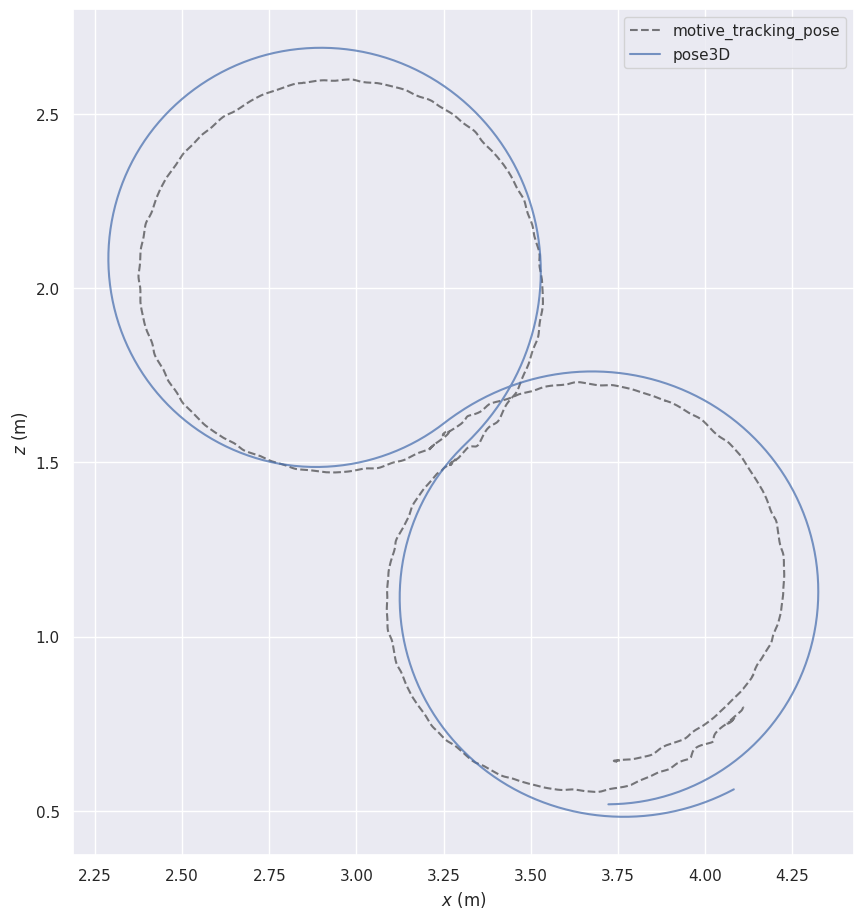
\includegraphics[width=0.5\textwidth]{figures/evo_pose3D.png}
    \caption{trajectories comparison between \texttt{pose3D} and ground truth (\texttt{motive\_tracking\_pose}) in the x-z plane.}
    \label{fig:pose3D_traj}
\end{figure}
\begin{figure}[H]
    \centering
    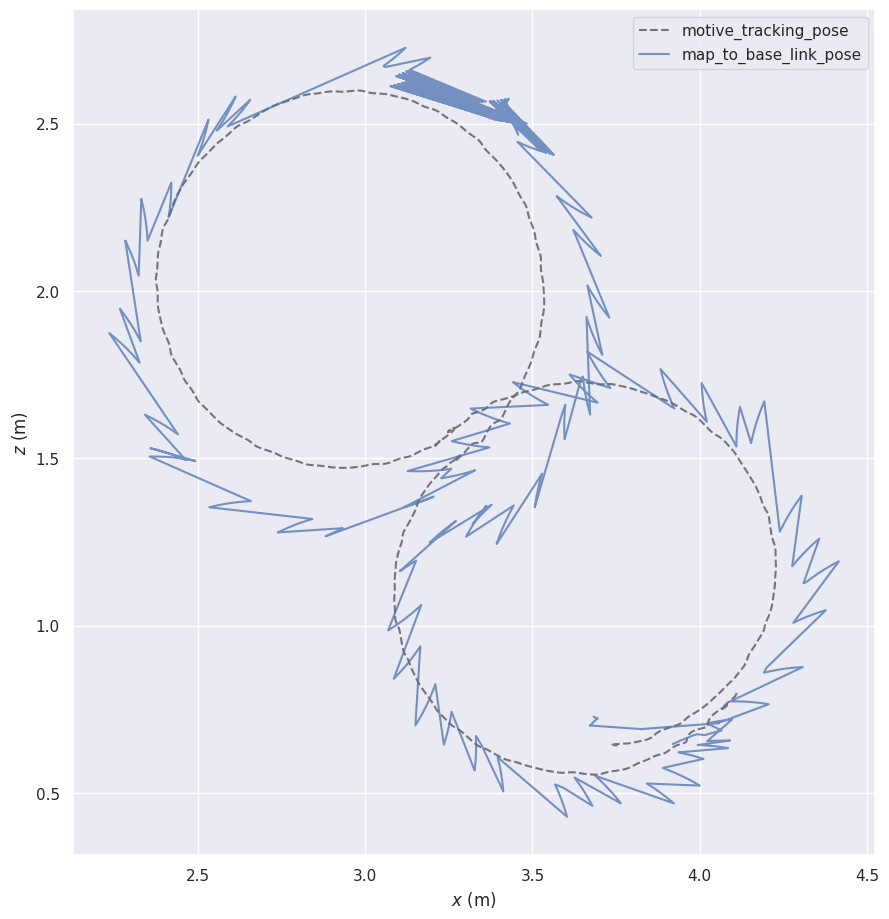
\includegraphics[width=0.5\textwidth]{figures/evo_mapping.png}
    \caption{trajectories comparison between \texttt{mapping} and ground truth (\texttt{motive\_tracking\_pose}) in the x-z plane.}
    \label{fig:mapping_traj}
\end{figure}
\begin{figure}[H]
    \centering
    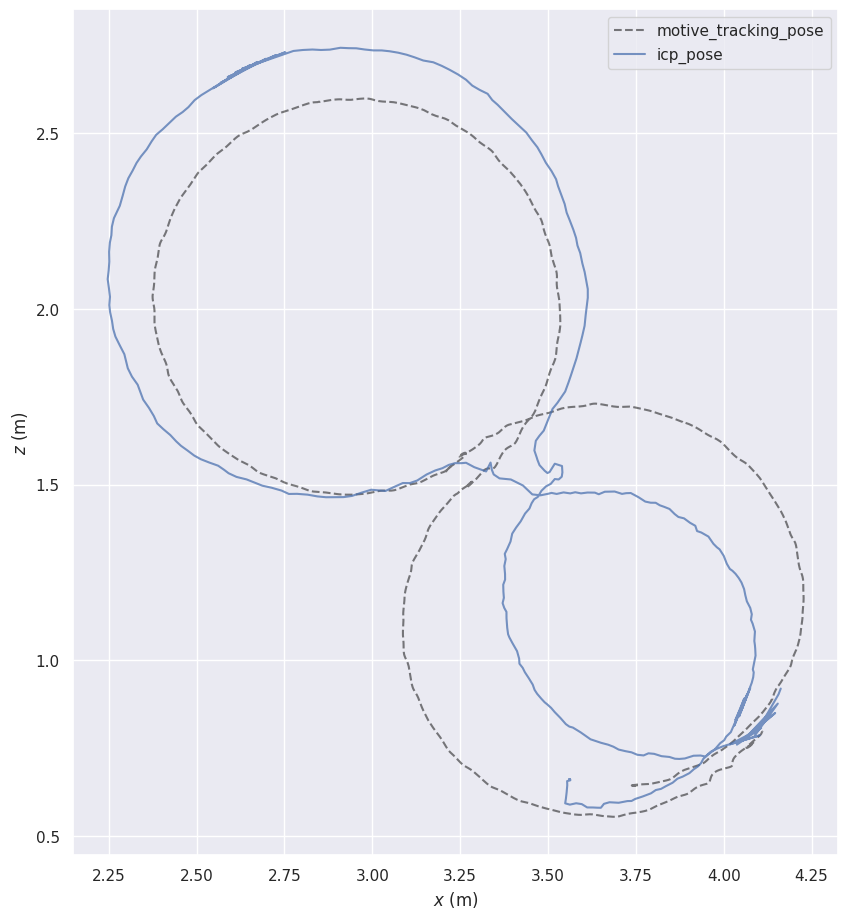
\includegraphics[width=0.5\textwidth]{figures/evo_icp.png}
    \caption{trajectories comparison between \texttt{icp} and ground truth (\texttt{motive\_tracking\_pose}) in the x-z plane.}
    \label{fig:icp_traj}
\end{figure}

\FloatBarrier % 确保以上图片和文字分组

Figures show the 2D projection of the estimated and ground truth trajectories in the x-z plane. The estimated path follows a figure-eight pattern, which is mostly consistent with the reference trajectories. However, some slight deviations can be observed, particularly around curved segments, indicating moderate drift or estimation error. This deviation may be caused by odometry noise or limited sensor fusion.

\section{Orientation Analysis}

\begin{figure}[H]
    \centering
    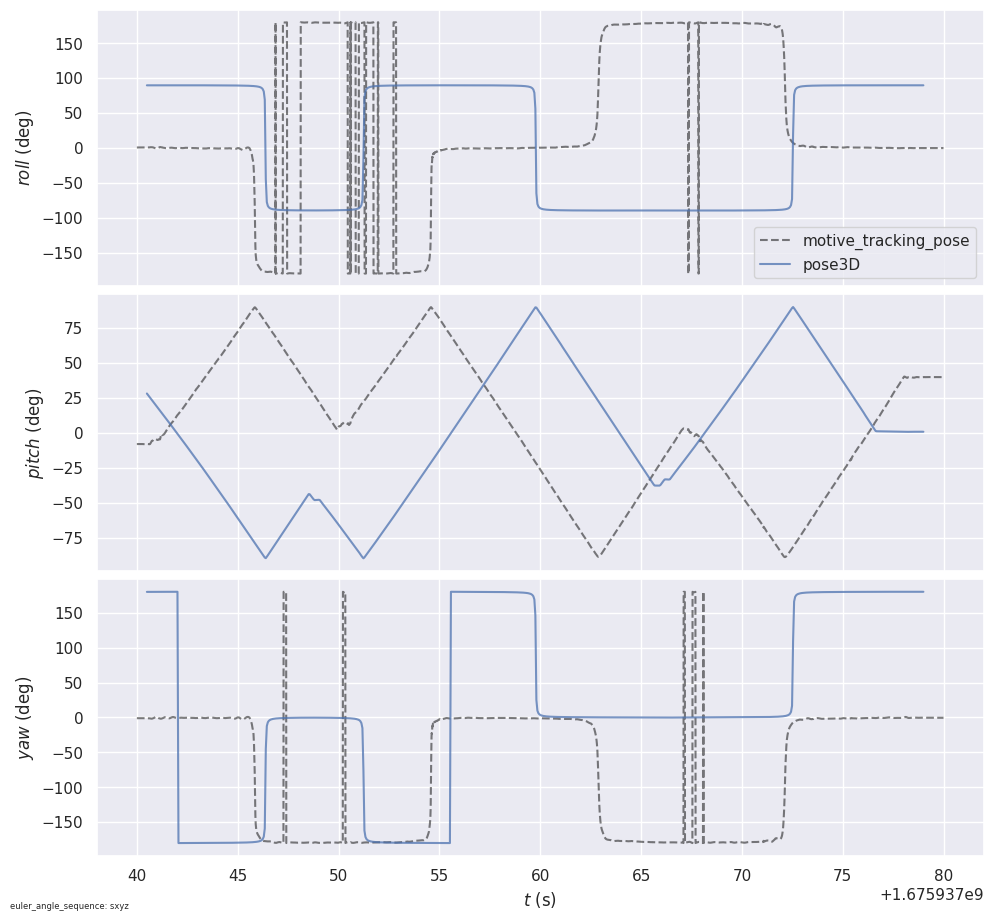
\includegraphics[width=0.5\textwidth]{figures/evo_pose3D_rpy.png}
    \caption{Orientation over time for \textbf{pose3D} estimated and ground truth trajectories.}
    \label{fig:pose3D_rpy}
\end{figure}
\begin{figure}[H]
    \centering
    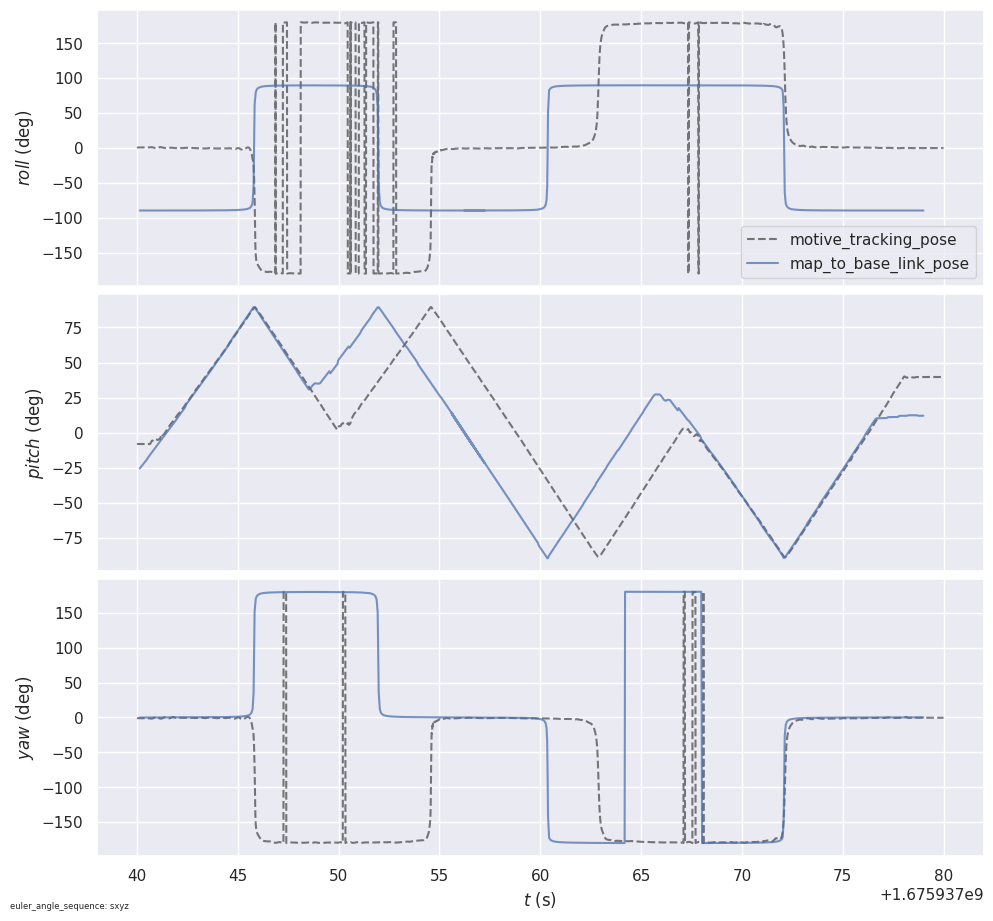
\includegraphics[width=0.5\textwidth]{figures/evo_mapping_rpy.png}
    \caption{Orientation over time for \textbf{mapping} estimated and ground truth trajectories.}
    \label{fig:mapping_rpy}
\end{figure}
\begin{figure}[H]
    \centering
    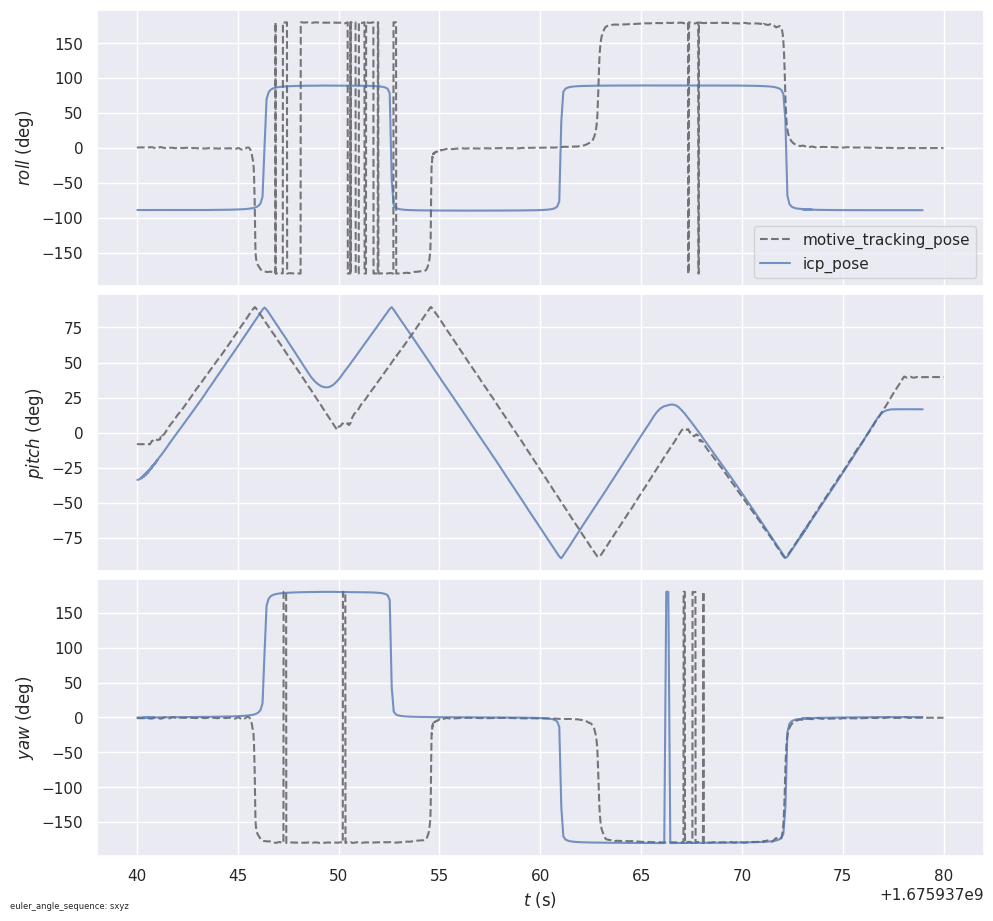
\includegraphics[width=0.5\textwidth]{figures/evo_icp_rpy.png}
    \caption{Orientation over time for \textbf{icp} estimated and ground truth trajectories.}
    \label{fig:icp_rpy}
\end{figure}

\FloatBarrier % 确保以上图片和文字分组

In Figures, roll, pitch, and yaw angles are plotted as a function of time. The estimated results displays smoother angular transitions, while the ground truth trajectories shows more high-frequency components and rapid variations. These spikes may be caused by fast motion changes or motion capture system noise. Notably, there are clear discrepancies in the roll and yaw components, which may be improved with better sensor alignment or orientation filtering.

\section{Position Over Time}

\begin{figure}[H]
    \centering
    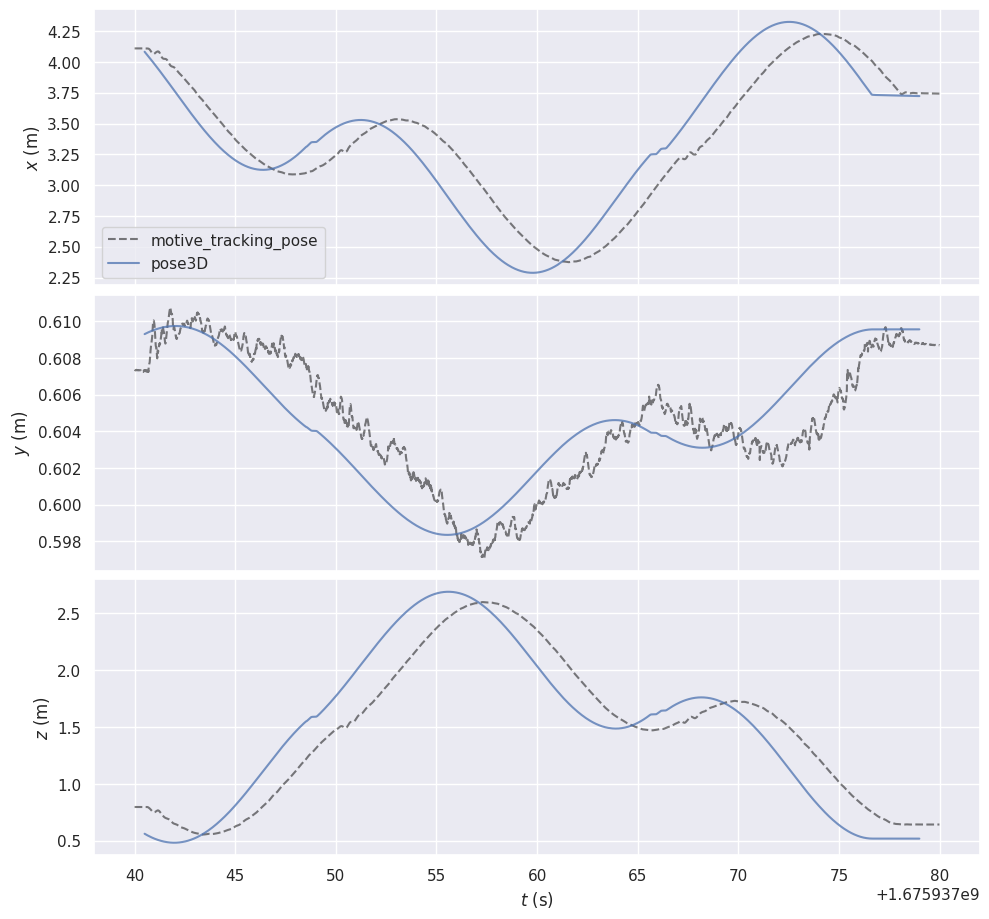
\includegraphics[width=0.5\textwidth]{figures/evo_pose3D_xyz.png}
    \caption{Position components ($x$, $y$, $z$) over time for pose3D.}
    \label{fig:pose3D_xyz}
\end{figure}
\begin{figure}[H]
    \centering
    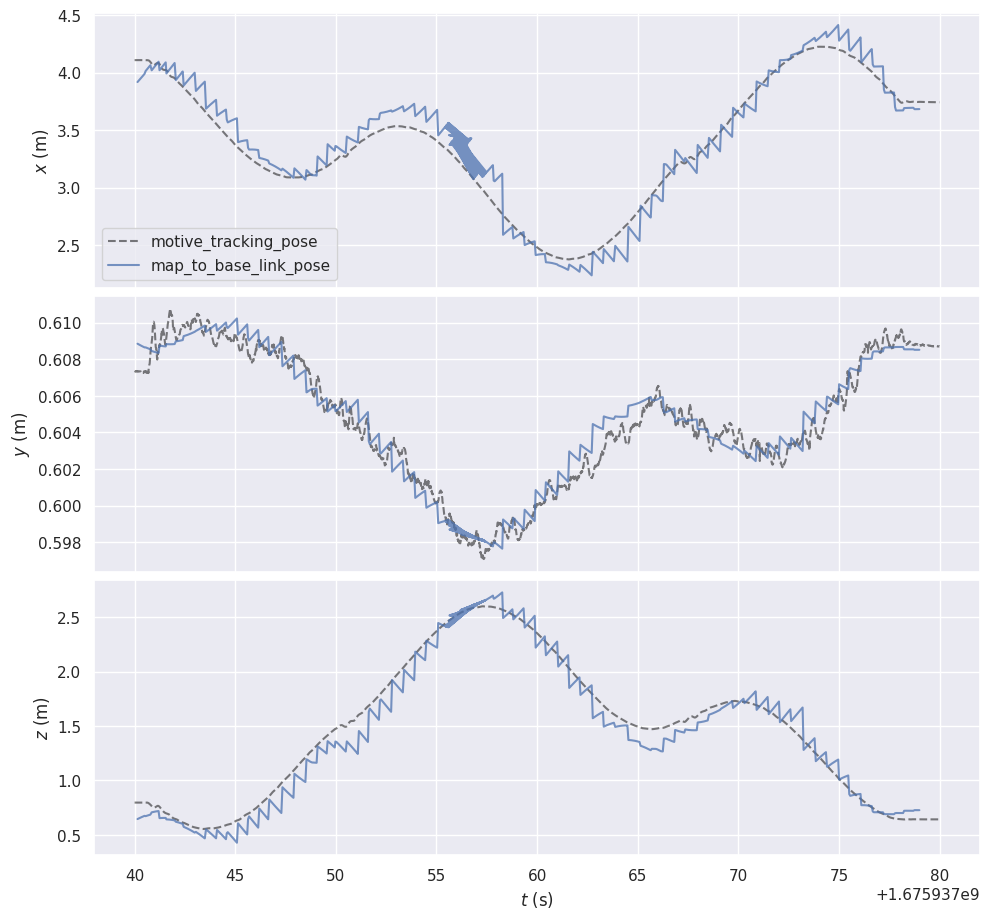
\includegraphics[width=0.5\textwidth]{figures/evo_mapping_xyz.png}
    \caption{Position components ($x$, $y$, $z$) over time for mapping.}
    \label{fig:mapping_xyz}
\end{figure}
\begin{figure}[H]
    \centering
    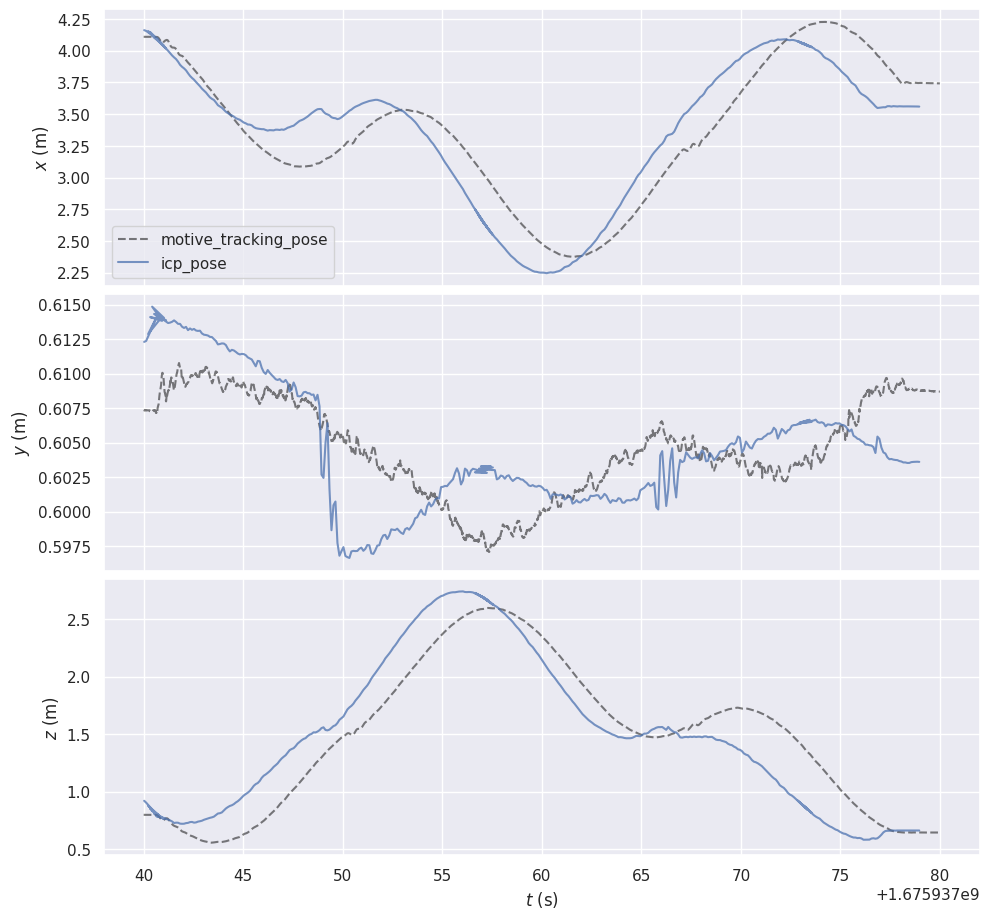
\includegraphics[width=0.5\textwidth]{figures/evo_icp_xyz.png}
    \caption{Position components ($x$, $y$, $z$) over time for icp.}
    \label{fig:icp_xyz}
\end{figure}

\FloatBarrier % 确保以上图片和文字分组

Figures displays the position evolution in each coordinate axis. The $x$ and $z$ components demonstrate good agreement between the estimated and ground truth values, with the estimate tracking the overall shape and dynamics accurately. The $y$ component, however, shows more noise in the ground truth data, which may be due to lateral vibrations or inaccuracies in the motion capture setup. Despite this, the  trajectories remains relatively stable and captures the correct trend.

\section{Conclusion}

The evaluation results suggest that the \texttt{pose3D} system performs well in estimating 3D position and orientation. While there are minor discrepancies, especially in orientation and during curves, the system is able to maintain a reasonable alignment with the ground truth. Further improvements could be achieved by refining sensor fusion strategies and enhancing time synchronization with the motion capture system.

\end{document}
